\documentclass[a4]{scrartcl}

% \usepackage[ngerman]{babel}
\usepackage[utf8]{inputenc}
\usepackage{mathtools}
\usepackage{amsmath}
\usepackage{amssymb}
\usepackage{geometry}
\usepackage{scrlayer-scrpage}
\pagestyle{scrheadings}
\usepackage{tablefootnote}
\usepackage[dvipsnames]{xcolor}
% \clearscrheadfoot

\setlength{\parindent}{0em}

\setlength{\parskip}{1.3ex}

\usepackage[onehalfspacing]{setspace}


\clubpenalty = 10000
\widowpenalty = 10000
\displaywidowpenalty = 10000

\usepackage{hyperref}
\hypersetup{
	colorlinks=true,
	linkcolor=black,
	filecolor=black,      
	urlcolor=BurntOrange,
	citecolor=black
}


\geometry{
	paper=a4paper, % Change to letterpaper for US letter
	top=3cm, % Top margin
	bottom=3cm, % Bottom margin
	left=2cm, % Left margin
	right=3cm, % Right margin
	%showframe, % Uncomment to show how the type block is set on the page
}

\usepackage[backend=biber, maxbibnames=99]{biblatex}
\addbibresource{references.bib}
\setcounter{biburllcpenalty}{7000}
\setcounter{biburlucpenalty}{8000}



\usepackage[framemethod=TikZ]{mdframed}

% Style %
\mdfdefinestyle{enviStyle}{
	innertopmargin = 10pt,
	linewidth      = 1pt,
	frametitlerule = true,
	roundcorner    = 2pt%
}


\usepackage{sectsty}
\sectionfont{\color{BurntOrange}}
\subsectionfont{\color{BurntOrange}}


\newenvironment{CountingDefinition}[2][]{%
	\ifstrempty{#1}%
	{\mdfsetup{%
			frametitle={{\strut ~}}}
	}%
	{\mdfsetup{%
			frametitle={{\strut ~#1}}}%
	}%
	\mdfsetup{
		nobreak                   = true,
		linecolor                 = BurntOrange,
		frametitlebackgroundcolor = BurntOrange!50,
		style                     = enviStyle
	}
	\begin{mdframed}[]\relax%
		\label{#2}}{\end{mdframed}}



\renewcommand{\labelitemi}{$\textcolor{BurntOrange}{\bullet}$}
\renewcommand{\labelitemii}{$\textcolor{BurntOrange}{\cdot}$}
\renewcommand{\labelitemiii}{$\textcolor{BurntOrange}{\diamond}$}
\renewcommand{\labelitemiv}{$\textcolor{BurntOrange}{\ast}$}





%\ohead{\\
%	Pina Kolling\\
%	piko0011}

\begin{document}
	
	\begin{titlepage}
		\centering
		{\scshape\LARGE Umeå University \par}
		\vspace{1cm}
		{\scshape\Large Managing the Digital Enterprise \par }
		\vspace{1.5cm}
		{\huge\bfseries   {\color{BurntOrange}Individual Assignment 3} \par}
		\vspace{2cm}
		{\Large\itshape Pina Kolling\par}
		\vfill
		supervised by \par 
		\vspace{1cm}
		Dr. Daniel \textsc{Skog} \par 
		and \par 
		M. Sc. Ramy \textsc{Shenouda} 
		
		\vfill
		
		% Bottom of the page
		{\large \today\par}
	\end{titlepage}
	
	\setcounter{page}{1}
	
	\begin{doublespace}
		\tableofcontents
	\end{doublespace}

	
	\newpage


% Two books in the course literature present and prescribe ways for organizations to manage digital transformation in useful ways. In order to make informed decisions as a manager of a digital enterprise of how to understand, evaluate, and potentially use different prescriptive statements, concepts, models or frameworks, a manager needs to be able to analyze and understand core assumptions underlying normative suggestions for action. For example, management literature tend to based on certain assumptions regarding who the reader is, what type of organization the person is in, what part of the world the organization operates, and prescribes advice accordingly. Your task is to:

%Identify core assumptions in Venkatraman (2017) and in Westerman et al. (2014).
%Discuss the consequences of these assumptions in terms of how digital transformation and approaches to managing it are portrayed in the two books.
%Use the results of 1 and 2, and your own example of an organization and context, to describe where, when and why the approach of either Venkatraman or Westerman et al, would not be suitable












%Identify core assumptions in Venkatraman (2017) and in Westerman et al. (2014).
%-------------------------------------------------------------------------------------------
	\section{Core assumptions in digital transformation literature} \label{sec:Sec1}
	
	In this Section, the core assumptions of Venkatraman in \textit{The digital matrix: new rules for business transformation through technology} \cite{leadingdigital} and Westerman, Bonnet and McAfee in \textit{Leading digital: Turning technology into business transformation} \cite{digitalmatrix} are presented.

%-------------------------------------------------------------------------------------------
% \subsection{Introduction of the authors} \label{subsec:authors}


	\begin{CountingDefinition}[Author of \textit{The digital matrix}]{def:defdef1}
		
		\begin{minipage}{0.3\linewidth}			
				\centering
				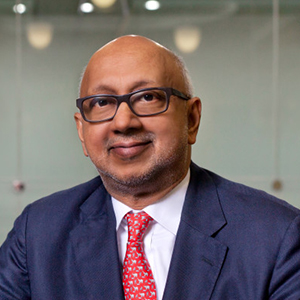
\includegraphics[width=0.65\textwidth]{images/VV.jpg}
				
				\tiny{Picture of Venkat Venkatraman\footnotemark} 
					
		\end{minipage}	\begin{minipage}{0.7\linewidth}
		
			Dr. Venkatraman holds a PhD from the University of Pittsburgh's (Katz Graduate School of Business, 1985). He specializes in the study of how established companies adapt to digital technologies. He published his knowledge in his book \textit{The Digital Matrix: New Rules for Business Transformation through Technology} in 2017. \cite{VV, digitalmatrix} 
		\end{minipage}

	
				
	\end{CountingDefinition}

	\footnotetext{Picture from \url{https://www.dukece.com/people/venkat-venkatraman/}}


	\begin{CountingDefinition}[Authors of \textit{Leading digital}]{def:defdef2}
		
		
		\begin{minipage}{0.3\linewidth}			
			\centering
			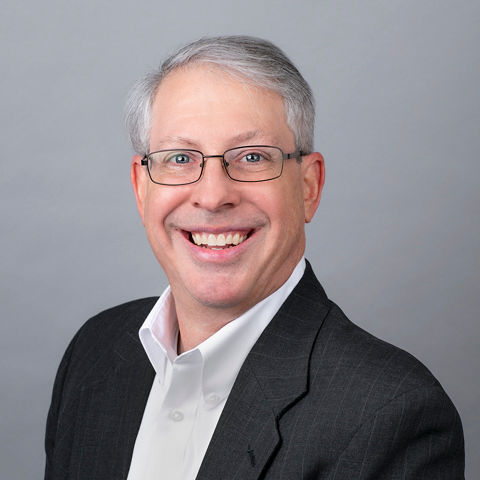
\includegraphics[width=0.5\textwidth]{images/GW.jpeg}
	
			\tiny{Picture of George Westermann\footnotemark} 
	
		\end{minipage}	\begin{minipage}{0.7\linewidth}
	
			George Westerman is a Senior Lecturer at MIT Sloan School of Management and Founder of the Global Opportunity Initiative. He has written award-winning books and conducted research on digital transformation. \cite{GW, leadingdigital}
			
		\end{minipage}



		\begin{minipage}{0.3\linewidth}			
			\centering
			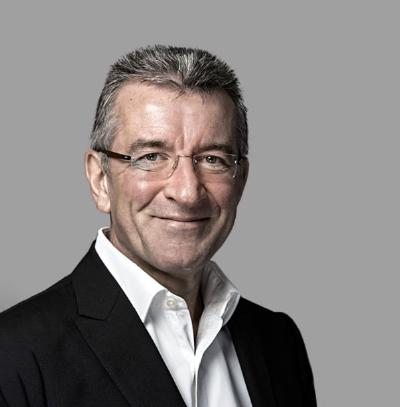
\includegraphics[width=0.5\textwidth]{images/DB.jpg}
	
			\tiny{Picture of Didie Bonnet\footnotemark} 
	
		\end{minipage}	\begin{minipage}{0.7\linewidth}
	
			Dr. Didier Bonnet is specialized on digital transformation. He is a Professor at IMD Business School (Switzerland) and co-author of the book \textit{Leading digital}. He is featured on broadcasts like the BBC or CNN. \cite{DB2, DB1, leadingdigital}
			
		\end{minipage}


		\begin{minipage}{0.3\linewidth}			
			\centering
			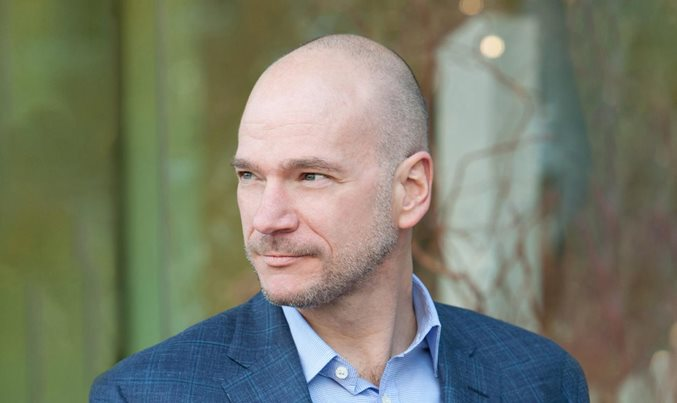
\includegraphics[width=0.65\textwidth]{images/AM.jpg}
	
			\tiny{Picture of Andrew McAfee\footnotemark} 
	
		\end{minipage}	\begin{minipage}{0.7\linewidth}
	
			Andrew McAfee is a principal research scientist at MIT and co-founder of the MIT Initiative on the Digital Economy. He has written numeral books, including \textit{Race Against the Machine}, \textit{The Second Machine Age} and \textit{Leading digital}. \cite{AM2, AM3, AM1, leadingdigital}
			
		\end{minipage}



		
	\end{CountingDefinition}

	\footnotetext{Picture from \url{https://mitsloan.mit.edu/faculty/directory/george-f-westerman}}
	\footnotetext{Picture from \url{https://digitaltransformation2021.brightline.org/speakers/didier-bonnet/}}
	\footnotetext{Picture from \url{https://www.mckinsey.com/capabilities/strategy-and-corporate-finance/our-insights/the-strategy-and-corporate-finance-blog/leadership-rundown-is-technology-a-force-for-good}}












%Discuss the consequences of these assumptions in terms of how digital transformation and approaches to managing it are portrayed in the two books.
%-------------------------------------------------------------------------------------------
\section{Consequences of assumptions in digital transformation} \label{sec:Sec2}

\begin{CountingDefinition}[Definitions]{def:defdef}
	
	\begin{tabular}{lp{13.5cm}}
		
		Text
		
	\end{tabular}
	
	
\end{CountingDefinition}






















%Use the results of 1 and 2, and your own example of an organization and context, to describe where, when and why the approach of either Venkatraman or Westerman et al, would not be suitable
%-------------------------------------------------------------------------------------------
\section{Constraints of conventional approaches} \label{sec:Sec3}

\begin{CountingDefinition}[Definitions]{def:defdef}
	
	\begin{tabular}{lp{13.5cm}}
		
		Text
		
	\end{tabular}
	
	
\end{CountingDefinition}




	
	\newpage
	\addcontentsline{toc}{section}{References}
	\begin{spacing}{0.9}
		\printbibliography
	\end{spacing}


	
	
	
	
	
	
\end{document}